\section{Results}
\label{sec:results}

\begin{table*}[t]
  \centering
  \caption{Citation $F_1$ by hop stratum in four settings. v2 and v3: DO-178C with the e5-small and text-embedding-3-small embedders (4{,}440 runs each). MuSiQue: 200 queries with the v3 embedder (600 runs; vanilla, agentic+graph, and GraphRAG only). 2Wiki: 200 2WikiMultihopQA queries at three seeds (1{,}200 runs; vanilla and GraphRAG only). Bold marks the best pipeline per setting and stratum.}
  \label{tab:dominance}
  \footnotesize\setlength{\tabcolsep}{3pt}
  \resizebox{\textwidth}{!}{%
  \begin{tabular}{l ccc | ccc | ccc | ccc}
    \toprule
     & \multicolumn{3}{c|}{v2 main (local)} & \multicolumn{3}{c|}{v3 main (Azure)} & \multicolumn{3}{c|}{MuSiQue (Azure)} & \multicolumn{3}{c}{2Wiki (Azure)} \\
    System & 1h & 2h & 3+h & 1h & 2h & 3+h & 1h & 2h & 3+h & 1h & 2h & 3+h \\
    \midrule
    vanilla & \textbf{.757} & .712 & .089 & \textbf{.756} & .689 & .195 & .742 & .415 & .277 & \textbf{.990} & .778 & .678 \\
    agentic & .541 & .414 & .175 & .533 & .430 & .203 & --- & --- & --- & --- & --- & --- \\
    agentic-graph & .566 & .415 & \textbf{.219} & .547 & .421 & .251 & .457 & .296 & .249 & --- & --- & --- \\
    graphrag & .751 & \textbf{.720} & .172 & .745 & \textbf{.707} & .253 & \textbf{.841} & \textbf{.632} & \textbf{.463} & .969 & \textbf{.946} & \textbf{.938} \\
    adaptive & .630 & .499 & .181 & .651 & .492 & \textbf{.254} & --- & --- & --- & --- & --- & --- \\
    \bottomrule
  \end{tabular}}
\end{table*}


\begin{figure}[t!]
  \centering
  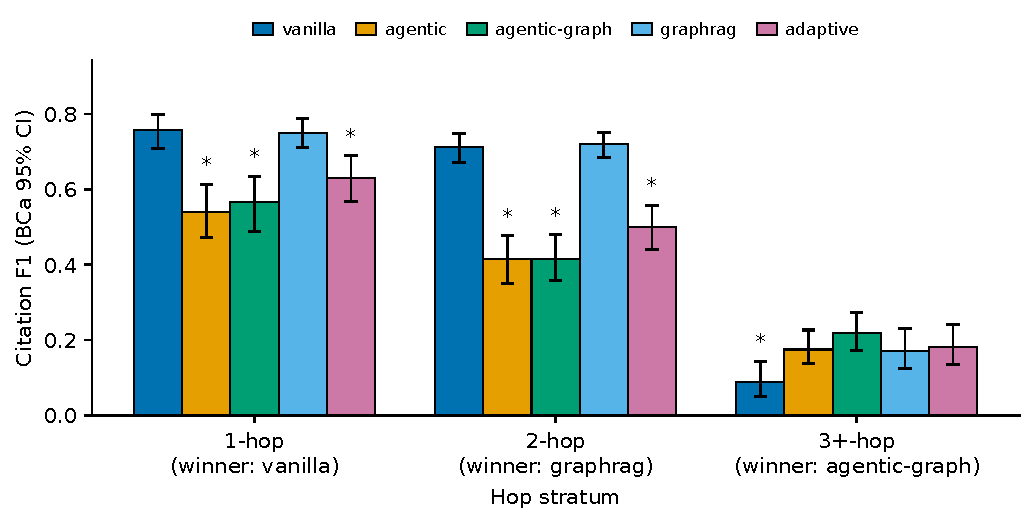
\includegraphics[width=0.55\textwidth]{figures/fig1_per_stratum_f1.pdf}
  \caption{Citation $F_1$ by hop stratum on the v2 matrix (DO-178C,
    e5-small), with 95\% BCa intervals. An asterisk marks a pipeline that
    differs significantly from the best pipeline in its stratum (Holm-adjusted
    Wilcoxon $p < 0.05$ and $|\delta| \ge 0.147$).}
  \label{fig:perstratum}
\end{figure}

\subsection{Citation Quality by Hop Depth (RQ1)}
\label{sec:c1}
Table~\ref{tab:dominance} reports citation $F_1$ by stratum in four
settings. On DO-178C, vanilla and GraphRAG are statistically tied on
one- and two-hop queries (Wilcoxon $p = 0.12$ and $0.65$ under the v2
embedder, with negligible $\delta$), and the agentic loop costs 0.19 to
0.30 $F_1$ on these strata. On queries of three or more hops the
ordering reverses. Vanilla falls to last place, and the pipelines that
use the graph lead; under the v2 embedder agentic+graph reaches 0.219
against 0.089 for vanilla (Holm $p < 10^{-6}$). Under the v3 embedder the ordering is the same, but no pair at this depth passes the joint criterion. Under bge-m3 the pattern recurs (Table~\ref{tab:embedders}):
vanilla is last at three or more
hops under all three embedders, and under bge-m3 both graph pipelines
outperform it by 0.100 and 0.091 (Holm $p = 2.1 \times 10^{-4}$ and
$1.4 \times 10^{-3}$), while the one- and two-hop contrasts remain
negligible.

On MuSiQue, GraphRAG is best in every stratum ($F_1$ of 0.841, 0.632,
and 0.463), with $p \le 5.1 \times 10^{-4}$ and $\delta$ between 0.27
and 0.43 against vanilla. Because the MuSiQue \textit{REFERENCES} edges
connect only gold paragraphs, we also ran GraphRAG on a graph with
additional edges between consecutive distractor paragraphs. GraphRAG
then loses 0.02, 0.05, and 0.09 $F_1$ per stratum and still outperforms
vanilla in every stratum ($p \le 0.014$), so its advantage on MuSiQue
does not depend on gold-only edges. On 2WikiMultihopQA, the two
pipelines are tied on one-hop queries ($p = 0.15$), and GraphRAG leads
on two-hop and deeper queries by 0.168 and 0.260 ($\delta = 0.48$ and
0.87). This is the DO-178C crossover again, on a graph we did not build.

Seed variation is small by comparison. The mean $F_1$ of each pipeline
changes by at most 0.031 between seeds,
every significant ordering holds in each seed separately, and the only
changes in rank occur between vanilla and GraphRAG on one- and two-hop
queries, which we already report as ties. Regarding RQ1, the best
pipeline depends on hop depth and on the corpus, but not on the embedder
or the seed.

\begin{table}[t]
  \centering
  \caption{Citation $F_1$ by hop stratum on DO-178C under three embedders from three vendors (e5-small, 384 dimensions; text-embedding-3-small, 1536; bge-m3, 1024). Bold marks the best pipeline per embedder and stratum.}
  \label{tab:embedders}
  \small
  \setlength{\tabcolsep}{4pt}
    \begin{tabular}{l rrr rrr rrr}
    \toprule
    & \multicolumn{3}{c}{e5-small (384d)} & \multicolumn{3}{c}{3-small (1536d)} & \multicolumn{3}{c}{bge-m3 (1024d)} \\
    \cmidrule(lr){2-4}\cmidrule(lr){5-7}\cmidrule(lr){8-10}
    System & 1h & 2h & 3+h & 1h & 2h & 3+h & 1h & 2h & 3+h \\
    \midrule
    vanilla       & \textbf{.757} & .712 & .089 & \textbf{.756} & .689 & .195 & \textbf{.769} & .691 & .114 \\
    agentic       & .541 & .414 & .175 & .533 & .430 & .203 & .548 & .404 & .156 \\
    agentic-graph & .566 & .415 & \textbf{.219} & .547 & .421 & .251 & .546 & .431 & .206 \\
    graphrag      & .751 & \textbf{.720} & .172 & .745 & \textbf{.707} & .253 & .742 & \textbf{.728} & \textbf{.214} \\
    adaptive      & .630 & .499 & .181 & .651 & .492 & \textbf{.254} & .672 & .478 & .202 \\
    \bottomrule
  \end{tabular}
\end{table}


\begin{table}[t]
  \centering
  \caption{Context and citation precision of GraphRAG in six settings. Slots: chunks passed to the synthesizer. IDs: IDs cited in the answer. Gain: citation precision divided by context precision.}
  \label{tab:pathology}
  \small
  \setlength{\tabcolsep}{4pt}
  \begin{tabular}{l rr rr r}
    \toprule
    & \multicolumn{2}{c}{\textit{retrieved context}} & \multicolumn{2}{c}{\textit{answer citations}} & \\
    \cmidrule(lr){2-3}\cmidrule(lr){4-5}
    Setting & slots & prec. & IDs & prec. & gain \\
    \midrule
    DO-178C, e5-small     & 14.9 & 0.120 & 4.9 & 0.480 & 4.0$\times$ \\
    DO-178C, 3-small      & 14.9 & 0.129 & 5.0 & 0.493 & 3.8$\times$ \\
    DO-178C, bge-m3       & 14.8 & 0.121 & 4.7 & 0.490 & 4.1$\times$ \\
    DO-178C, PPR walk     & 14.9 & 0.131 & 4.9 & 0.509 & 3.9$\times$ \\
    MuSiQue               & 11.2 & 0.227 & 3.4 & 0.654 & 2.9$\times$ \\
    2WikiMultihopQA       & 11.4 & 0.230 & 2.5 & 0.975 & 4.2$\times$ \\
    \bottomrule
  \end{tabular}
\end{table}


\begin{figure}[t!]
  \centering
  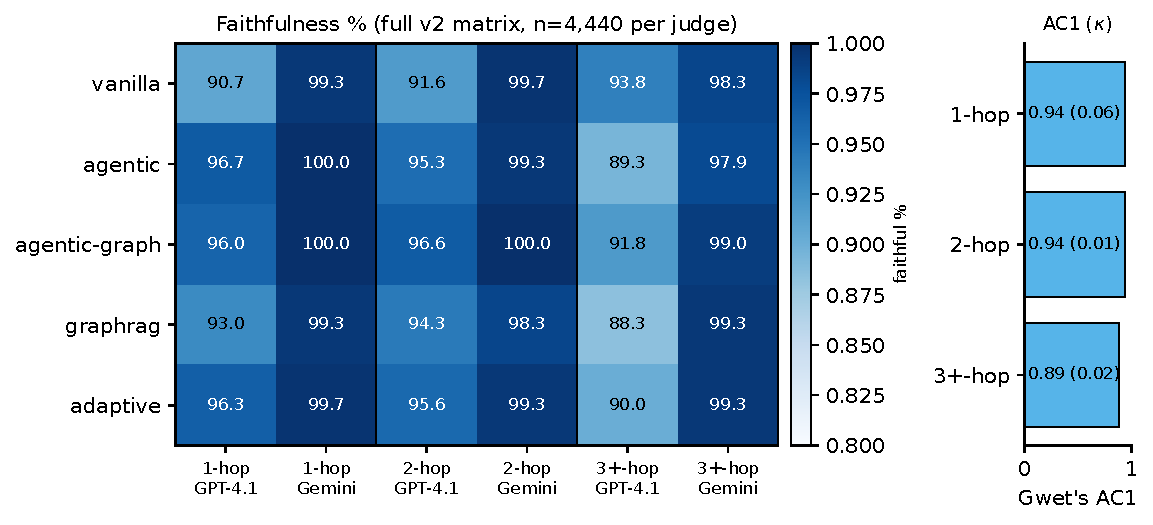
\includegraphics[width=0.8\textwidth]{figures/fig2_faithfulness_heatmap.pdf}
  \caption{Faithfulness on the full v2 matrix (DO-178C, e5-small; 4{,}440
    rows, about 300 per cell), judged by GPT-4.1 and Gemini 3.7-flash on
    the same rows. Left: percentage of answers judged faithful. Right:
    Gwet's AC1 between the two judges per stratum, with Cohen's $\kappa$
    in parentheses. The colour scale starts at 80\%.}
  \label{fig:faithheatmap}
\end{figure}

\subsection{Context Versus Answer Citations (RQ2)}
\label{sec:c2}
Table~\ref{tab:pathology} reports the same measurement in six settings,
covering three embedders, three corpora, and two traversals. GraphRAG's
walk fills 11 to 15 context slots at a context precision of 0.12 to
0.23, so four or five of every six chunks it retrieves are not gold. The
synthesizer then cites only 2.5 to 5.0 IDs per answer, at a citation
precision of 0.48 to 0.98. In every setting, the precision of the
citations is 2.9 to 4.2 times that of the context. The $F_1$ advantage
of GraphRAG is therefore a recall effect: the walk retrieves gold chunks
that dense retrieval misses, and the synthesizer does not cite most of
the irrelevant chunks that come with them.

An evaluation that scores the retrieved set as the attribution set, as
some GraphRAG comparisons do, sees only the first step and reaches the
opposite ranking. By context precision, GraphRAG
is below the vanilla baseline in every setting (0.12 to 0.23, against
0.27 to 0.37 for vanilla). By citation $F_1$, it is the best pipeline in
every setting, with scores of 0.551, 0.571, 0.565, 0.585, 0.646, and
0.951 in the row order of Table~\ref{tab:pathology}. 

Two controls test whether this depends on our design. The first
replaces the two-hop walk with personalized PageRank over the same
graph. Context
precision is 0.131 with PageRank and 0.129 with the original walk (0.131
for the walk rebuilt on the same file-backed graph;
Section~\ref{sec:experiments}). The precision gain from context to
citations is 3.9 and 3.8 times, and the difference in citation $F_1$ is
0.016 with $\delta = 0.036$, which our criterion treats as negligible.
The second control applies two mitigations on MuSiQue. Reranking the
walked neighbours by similarity to the query and keeping the top five
changes little (context precision from 0.227 to 0.232, citation $F_1$
$+0.010$, $p = 0.34$). Reducing the traversal budget from 30 to 10 nodes
and the context from 15 to 8 chunks lowers citation $F_1$ by 0.126
($p = 2.6 \times 10^{-11}$) and also lowers context precision, to 0.194.
Both outcomes fit a synthesizer that already filters: an upstream
filter adds little, and a smaller budget removes the recall the
advantage depends on. Regarding RQ2, the comparison
reverses with the measurement point in all six settings.

\subsection{Faithfulness and Hop Depth (RQ3)}
\label{sec:c3}
On 300-row judged subsets, faithfulness declines with hop depth on
DO-178C but not on the Wikipedia chains. This difference disappears at
adequate power. The MuSiQue arm had 67 rows per
stratum. Its drop from one-hop to three-or-more-hop queries (9.2
percentage points) was larger than the 4.7-point drop that is
significant on DO-178C, but detecting it with 80\% power requires about
210 rows per cell. With three seeds ($n = 600$), the decline is
significant under both judges, from 0.930 to 0.876 to 0.823 under GPT-4.1
($p = 1.1 \times 10^{-3}$) and from 0.955 to 0.945 to 0.869 under Gemini
($p = 1.2 \times 10^{-3}$). On 2WikiMultihopQA, judged in full
($n = 1{,}200$), faithfulness also declines ($p = 5.0 \times 10^{-2}$ and
$4.8 \times 10^{-6}$). The decline therefore replicates on all three
corpora under two vendors.

What distinguishes the pipelines is whether they expand the context.
Vanilla retrieves a fixed top five and adds nothing, and under GPT-4.1
it shows no significant drop from one-hop to three-or-more-hop queries.
Its change is $-1.5$ points on DO-178C ($n = 2{,}072$; $p = 0.16$, 0.99,
and 0.76 for the three embedders) and $+1.1$ points on 2WikiMultihopQA
($p = 0.66$). The four expanding pipelines drop by 6.3 and 6.7 points on
the same corpora (Fig.~\ref{fig:faithheatmap}). A logistic regression
of faithfulness on hop depth, an expansion indicator, and their
interaction turns this contrast into a single test. The interaction is
negative and significant on the pooled DO-178C matrix ($b = -0.599$,
$p = 1.0 \times 10^{-7}$, $n = 10{,}360$), and negative but not
significant on 2WikiMultihopQA ($b = -0.286$, $p = 0.27$), whose arm is
one twentieth the size.

Under Gemini the ordering is the same, but the test does not resolve.
Near the ceiling, vanilla itself shows a slope ($b = -0.729$,
$p = 0.012$), and the interaction cannot be separated from it
($p = 0.11$). The expanding pipelines still drop more than vanilla (2.8
against 1.5 points on DO-178C, 12.7 against 7.7 on 2WikiMultihopQA). A lenient judge preserves the ranking but not the power to test it
(Section~\ref{sec:c4}). Not every expanding pipeline declines in every cell: GraphRAG is
marginal under bge-m3 ($p = 0.065$), and the agentic pipelines decline
in four of six embedder and pipeline combinations. We have not re-run the GPT-5.4
judge at this sample size. Regarding RQ3, faithfulness declines with
hop depth on every corpus, and the decline is steeper for pipelines
that expand their context.

\begin{table}[t]
  \centering
  \caption{Judge agreement. Top: the same judge re-judging identical answer and context strings, so only the date differs. Middle: the same judge after an embedder swap changes the input. Bottom: GPT-4.1 against Gemini 3.7-flash on identical rows; the last column gives the fraction judged faithful by each.}
  \label{tab:judges}
  \small
  \setlength{\tabcolsep}{4pt}
    \begin{tabular}{l rrrr}
    \toprule
    \multicolumn{5}{l}{\textit{Same judge, frozen input (answer + context identical)}} \\
    \midrule
    GPT-5.4, re-judged same day & \multicolumn{4}{r}{$\kappa = 0.764$, raw agr.\ 0.88} \\
    GPT-5.4, re-judged 11 wk later & \multicolumn{4}{r}{$\kappa = 0.138$, raw agr.\ 0.56} \\
    GPT-4.1, re-judged 11 wk later & \multicolumn{4}{r}{$\kappa = -0.05\,/\,-0.00$ (v2/v3), raw agr.\ 0.48\,/\,0.51} \\
    GPT-4.1, full matrix vs.\ May & \multicolumn{4}{r}{$\kappa = -0.046$, raw agr.\ 0.48, $+43$\,pp} \\
    \midrule
    \multicolumn{5}{l}{\textit{Same judge, input changed by embedder swap}} \\
    \midrule
    GPT-5.4 (v2 vs v3) & \multicolumn{4}{r}{$\kappa = 0.137$, raw agr.\ 0.59} \\
    GPT-4.1 (v2 vs v3) & \multicolumn{4}{r}{$\kappa = 0.480$, raw agr.\ 0.74} \\
    \midrule
    \multicolumn{5}{l}{\textit{Cross-vendor, same rows (Gemini 3.7-flash vs.\ GPT-4.1)}} \\
    \midrule
    \textit{Setting} & raw & $\kappa$ & AC1 & faithful (G\,/\,4.1) \\
    \midrule
    DO-178C e5-small ($n{=}4{,}440$) & 0.929 & 0.029 & 0.923 & 0.993 / 0.933 \\
    DO-178C 3-small ($n{=}4{,}440$)  & 0.913 & 0.125 & 0.903 & 0.980 / 0.917 \\
    DO-178C bge-m3 ($n{=}1{,}480$)   & 0.939 & 0.047 & 0.935 & 0.991 / 0.945 \\
    DO-178C PPR walk ($n{=}296$)     & 0.926 & 0.058 & 0.919 & 0.983 / 0.936 \\
    MuSiQue, 3 seeds ($n{=}600$)     & 0.850 & 0.172 & 0.817 & 0.923 / 0.877 \\
    MuSiQue rerank ($n{=}200$)       & 0.820 & 0.171 & 0.772 & 0.935 / 0.825 \\
    MuSiQue budget cap ($n{=}200$)   & 0.875 & 0.419 & 0.841 & 0.875 / 0.880 \\
    2WikiMultihopQA ($n{=}1{,}200$)  & 0.899 & 0.435 & 0.877 & 0.888 / 0.914 \\
    \bottomrule
  \end{tabular}
\end{table}


\subsection{Judge Stability (RQ4)}
\label{sec:c4}
Table~\ref{tab:judges} separates instability on fixed inputs from
instability after the retrieval state changes.
\textit{Fixed inputs.} Re-judging the same 300 stored answer and
context pairs gives GPT-5.4 a self-agreement of $\kappa = 0.76$ (raw
agreement 0.88) on the same day, but only $\kappa = 0.14$ (raw agreement
0.56) eleven weeks later, with 15 points more answers judged faithful.
This rejects a stationary judge (binomial $p < 10^{-44}$). GPT-4.1 on the same tuples agrees with its own earlier
verdicts only at chance level ($\kappa = -0.05$ and $-0.00$ for v2 and
v3) and judges 41 points more answers faithful. With fixed inputs, this is drift of the judge alone.
\textit{Changed retrieval state.} After an embedder swap, which
changes the context and the answer for 94\% of the tuples, GPT-5.4
changes 41\% of its verdicts ($\kappa = 0.137$) and GPT-4.1 changes 26\%
($\kappa = 0.48$). The judge that is more stable under the embedder
swap is thus the less stable over time.
\textit{Across vendors.} On the same rows, Gemini 3.7-flash is much
more lenient than GPT-4.1 on all four DO-178C settings (0.98 to 0.99
against 0.92 to 0.95 faithful; McNemar $p < 10^{-9}$). They are indistinguishable on the budget-capped MuSiQue arm (0.875 against 0.880,
$p = 1.00$), and Gemini is stricter on 2WikiMultihopQA (0.888 against
0.914, $p = 6.2 \times 10^{-3}$). Strictness is therefore a property of
the judge and corpus together, and a calibration offset measured on one
corpus cannot be reused on another. The same eight
settings show the prevalence paradox~\cite{feinstein1990} within one
pair of judges. Raw agreement ranges only from 0.82 to 0.94, and Gwet's
AC1 follows it (0.77 to 0.94), whereas $\kappa$ ranges from 0.03 to
0.44, ordered almost exactly by the distance of faithfulness from the
ceiling. On 2WikiMultihopQA the two judges agree less often than on
DO-178C (0.899 against 0.93), yet their $\kappa$ is fifteen times
higher (0.435 against 0.029). Leniency and trend are nevertheless
separate properties. Although Gemini is near the ceiling on DO-178C, it
reproduces the decline with hop depth on both DO-178C matrices
($p = 4.3 \times 10^{-3}$ and $p < 10^{-16}$) and on both Wikipedia
corpora. The ordering a judge induces replicates across vendors, while
its strictness does not.
\textit{Between judges.} Inter-judge agreement halves under the embedder swap ($\kappa$ from
0.30 to 0.17; McNemar $p < 0.001$), and on the 300-row MuSiQue batch
GPT-5.4 and GPT-4.1 agreed only at chance (raw agreement 0.48, AC1
0.08), a real disagreement rather than a prevalence effect. We therefore
re-judged the full matrix within one judging period
(Section~\ref{sec:c3}), and no comparison we report spans judging
dates. Regarding RQ4, judges are not stable over
time, across retrieval states, or across vendors, although the hop-wise
ordering they induce is.
